\iffalse
\def\mytitle{Convex-Optimization}
\def\myauthor{K.Pavan Kumar}
\def\contact{r170850@rguktrkv.ac.in}
\def\mymodule{Future Wireless Communication (FWC)}
\documentclass[10pt, a4paper]{article}
\usepackage[a4paper,outer=1.5cm,inner=1.5cm,top=1.75cm,bottom=1.5cm]{geometry}
\twocolumn
\usepackage{graphicx}
\graphicspath{{./images/}}
\usepackage[colorlinks,linkcolor={black},citecolor={blue!80!black},urlcolor={blue!80!black}]{hyperref}
\usepackage[parfill]{parskip}
\usepackage{lmodern}
\usepackage{tikz}
	\usepackage{physics}
\usepackage{tabularx}
\usepackage{enumitem}
\usetikzlibrary{calc}
\usepackage{amsmath}
\usepackage{amssymb}
\renewcommand*\familydefault{\sfdefault}
\usepackage{watermark}
\usepackage{lipsum}
\usepackage{xcolor}
\usepackage{listings}
\usepackage{float}
\usepackage{titlesec}
\providecommand{\mtx}[1]{\mathbf{#1}}
\titlespacing{\subsection}{1pt}{\parskip}{3pt}
\titlespacing{\subsubsection}{0pt}{\parskip}{-\parskip}
\titlespacing{\paragraph}{0pt}{\parskip}{\parskip}


\newcommand{\myvec}[1]{\ensuremath{\begin{pmatrix}#1\end{pmatrix}}}
\let\vec\mathbf
\lstset{
frame=single, 
breaklines=true,
columns=fullflexible
}
\thiswatermark{\centering \put(0,-110.0){
\includegraphics[scale=0.3]{logo.png}} }
\title{\mytitle}
\author{\myauthor\hspace{1em}\\\contact\\FWC22011\hspace{6.5em}IITH\hspace{0.5em}\mymodule\hspace{6em}Optimization:Basic}
\date{}
\begin{document}
	\maketitle
	\tableofcontents
   \section{Problem}
   \fi
Maximise 
\begin{align}
Z = – x + 2y
\end{align}
 subject to the constraints
\begin{align}
	x + y &\geq 5
	\\
	x + 2y &\geq 6
	\\
	x \geq 3, y &\geq 0.
\end{align}
	\begin{figure}[!ht]
		\centering
		\includegraphics[width=\columnwidth]{12/12/1/9/figs/image.png}
		\caption{}
		\label{fig:12/12/1/9}
  	\end{figure}
\solution
The given problem can be expressed as
\begin{align}
z = \max_\vec{x}\myvec{-1 &2}\vec{x}
\\
s.t. \quad
    \myvec{1&1\\1&2\\1&0\\0&1}\vec{x}=\myvec{5\\6\\3\\0}
\end{align}
By providing the objective function and constraints to cvxpy, the optimal value gives infinity as result and the problem is unbounded.
This is verified from Fig. 
		\ref{fig:12/12/1/9}.
		\iffalse

\textbf{Reason:}
Unbounded means  if there exists some direction within the feasible region along which the objective function value can increase (maximization case) or decrease (minimization case) without bound. In such a formulation, the optimal value is negative infinity for a minimization problem, and conversely, positive infinity for a maximization problem.

An unbounded solution is something that typically does not arise in practical applications. When it does occur, it’s usually because the formulation is ill-posed, i.e., incorrect in some way, and/or missing some necessary constraints for properly modeling the dynamics of the system under consideration.

\vspace{20cm}
\textbf{termux commands :}
\begin{lstlisting}
bash basic.sh............using shell command
\end{lstlisting}

\textbf{cvxpy code:}
\begin{center}
\fbox{\parbox{8.5cm}{\url{https://github.com/FWC_module1/blob/main/optimization/basic.py}}}
\end{center}

\textbf{Graphical method:}
\begin{center}
   {\includegraphics[scale=0.5]{image.png}}  
\end{center}
From Graph,
\begin{center}
\begin{tabular}{|c|c|}
	\hline
	corner points&z\\
	\hline
	\textbf{(3,2)}&\textbf{1}\\
	\hline
    (4,1)&-2\\
    \hline
    (6,0)&-6\\
	\hline
\end{tabular}
\end{center}

Clearly the corner point (3,2) has maximum value for the given objective function.

But, as the feasible region is unbounded ,'\textbf{1}' may or may not be the maximum value. So ,we need to graph the inequality -x+2y $>$ 1.\\
$\because$ Feasible region of -x+2y $>$ 1 has some  points in common with the given constraints .so ,there is no maximum value for  z subject to given constraints.

\end{document}
\fi
